%%%%%%%%%%%%%%%%%%%%%%%%%%%%%%%%%%%%%%%%%%%%%%%%%%%%%%%%%%%%%%%%%%%%%%%%%%%%%%%%
%2345678901234567890123456789012345678901234567890123456789012345678901234567890
%        1         2         3         4         5         6         7         8

\documentclass[letterpaper, 10 pt]{IEEEconf}

\usepackage[utf8]{inputenc}
\usepackage[T1]{fontenc}

% The following packages can be found on http:\\www.ctan.org
%\usepackage{graphics} % for pdf, bitmapped graphics files
%\usepackage{epsfig} % for postscript graphics files
\usepackage{mathptmx} % assumes new font selection scheme installed
\usepackage{amsmath} % assumes amsmath package installed
\usepackage{amssymb}  % assumes amsmath package installed

\usepackage{tikz}
\usetikzlibrary{shapes.geometric, arrows, positioning, bending}


\usepackage{todonotes}

\title{\LARGE \bf
An Overview of reinforcement learning
}

\author{Emmanuel Madrigal% <-this % stops a space
}


\begin{document}

\maketitle\todo{Fix title}

%%%%%%%%%%%%%%%%%%%%%%%%%%%%%%%%%%%%%%%%%%%%%%%%%%%%%%%%%%%%%%%%%%%%%%%%%%%%%%%%
\begin{abstract}

	This electronic document is a ``live'' template. The various components of your paper [title, text, heads, etc.] are already defined on the style sheet, as illustrated by the portions given in this document.\todo{Add correct abstract}

\end{abstract}

\section{What is it?}

Reinforcement learning is learning what to do to maximize a numerical
reward signal. The learner is not told which actions to take, but must
discover which actions yield the most reward by trying them. In the
most interesting and challenging cases, actions may affect not only
the immediate reward but also the next situation and, through that,
all subsequent rewards. These two characteristics (trial-and-error
search and delayed reward) are the two most important distinguishing
features of reinforcement learning~\cite{sutton2018reinforcement}.

Reinforcement learning differs from supervised learning which
comprises learning from a training set of labeled examples provided by
a knowledgeable external supervisor. Each example is a description of
a situation together with a specification—the label—of the correct
action the system should take to that situation. The object of
supervised learning is for the system to extrapolate, or generalize,
its responses so it acts correctly in situations not present in the
training set. In interactive problems it is often impractical to get
examples of desired behavior that are both correct and representative
of all the situations in which the agent has to act. In uncharted
territory (where learning to be most beneficial), an agent must be
able to learn from its own experience~\cite{sutton2018reinforcement}.

Reinforcement learning is also different from what machine learning
researchers call unsupervised learning, which is typically about
finding structure hidden in collections of unlabeled
data. Reinforcement learning is trying to maximize a reward signal
instead of trying to find hidden structure. Uncovering structure in an
agent’s experience can be useful in reinforcement learning, but by
itself does not address the reinforcement learning problem of
maximizing a reward signal~\cite{sutton2018reinforcement}.

\section{What are its principles?} % Cuales son sus principios

\begin{figure}
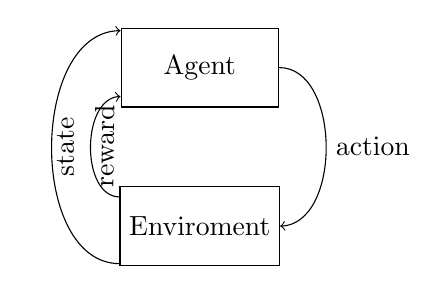
\begin{tikzpicture}[node distance=1cm]
  \node (agent) [rectangle,
    minimum width=2cm,
    minimum height=1cm,
    text centered,
    draw=black] {Agent};
  
  \node (env) [rectangle,
    minimum width=2cm,
    minimum height=1cm,
    text centered,
    draw=black,
  below = of agent] {Enviroment};

  \draw[bend left=90,->]  (agent.east) to node [auto] {action} (env.east);
  
  \draw[bend right=90,<-]  (agent.200) to node [auto, below=0.5em, sloped, anchor=center] {reward} (env.160);
  \draw[bend right=90,<-]  (agent.155) to node [auto, below=0.5em, sloped, anchor=center] {state} (env.205);  
\end{tikzpicture}
\caption{Machine learning system}
\end{figure}

\subsection{Agent and Enviroment}

Reinforcement learning involves an interaction between an active
decision-making agent and its environment, within
which the agent seeks to achieve a goal despite uncertainty about its
environment. The agent’s actions may affect the future state of the
environment (e.g., the next chess position, the level of reservoirs of
the refinery, the robot’s next location and the future charge level of
its battery), affecting the options and opportunities available to the
agent at later times. Correct choice requires taking into account
indirect, delayed consequences of actions, and thus may require
foresight or planning. The effects of actions cannot be fully
predicted; thus the agent must monitor its environment frequently and
react appropriately. Use cases for reinforcement learning involve
explicit goals in the sense that the agent can judge progress toward
its goal based on what it can sense directly~\cite{sutton2018reinforcement}.

\subsection{Policy}

A policy defines the learning agent’s way of behaving given a
situation or state. Roughly, a policy is a mapping from perceived
states of the environment to actions to take when in those
states. Sometimes the policy may be a simple function or lookup table,
whereas in others it may involve extensive computation such as a
search process. The policy is the core of a reinforcement learning
agent in the sense that it alone suffices to determine behavior.  A
reward signal defines the goal in a reinforcement learning problem. On
each time step, the environment sends to the reinforcement learning
agent a single number called the reward. The agent’s sole aim is to
maximize the total reward it receives over the long run. The reward
signal thus defines what are the good and bad events for the
agent. They are the immediate and defining features of the problem
faced by the agent. The reward signal is the primary basis for
altering the policy; if an action selected by the policy results in a
low reward, then the policy may change to select some other action in
that situation. Reward signals may be stochastic functions of the
state of the environment and the actions taken~\cite{sutton2018reinforcement}.

\subsection{Reward and Value}

Whereas the reward signal shows what is good in an immediate sense, a
value function specifies what is good in the long run. Roughly, the
value of a state is the total amount of reward an agent can expect to
accumulate over the future, starting from that state. Whereas rewards
determine the immediate, intrinsic desirability of environmental
states, values show the long-term desirability of states after taking
into account the states that are likely to follow, and the rewards
available in those states. For example, a state might always yield a
low immediate reward but still have a high value because it is
regularly followed by other states that yield high rewards. Or the
reverse could be true.  Rewards are primary, whereas values, as
predictions of rewards, are secondary. Without rewards there could be
no values, and the only purpose of estimating values is to achieve
more reward. It is values with which we are most concerned when making
and testing decisions. Action choices are made based on value
judgments. We seek actions that bring about states of highest value,
not highest reward, because these actions result in the greatest
amount of reward for us over the long run. Unfortunately, it is much
harder to determine values than it is to determine rewards. Rewards
are given directly by the environment, but values must be estimated
and re-estimated from the sequences of observations an agent makes
over its entire lifetime. In fact, the most important component of
almost all reinforcement learning algorithms we consider is a method
for efficiently estimating values. The central role of value
estimation is arguably the most important thing we have learned about
reinforcement learning over the last few decades~\cite{sutton2018reinforcement}.

\subsection{Enviroment Model}

The fourth and final element of some reinforcement learning systems is
a model of the environment. This is something that mimics the behavior
of the environment, or that allows inferences to be made about how the
environment will behave. For example, given a state and action, the
model might predict the resultant next state and next reward. Models
are used for planning, by which we mean any way of deciding on a
course of action by considering possible future situations before they
are actually experienced. Methods for solving reinforcement learning
problems that use models and planning are called model-based methods,
as opposed to simpler model-free methods that are explicitly
trial-and-error learners—viewed as almost the opposite of planning~\cite{sutton2018reinforcement}.

\section{What algorithms exist?}

\todo{}

\subsection{Tabular Soltion Methods}

That in which the state and action spaces are small enough for the approximate value functions to be represented as arrays, or tables. In this case, the methods can often findexact solutions, that is, they can often find exactly the optimal value function and the optimal policy. This contrasts with the approximate methods described in the next section, which only find approximate solutions, but which in return can be applied effectively to much larger problems.

\subsubsection{Q-Learning}

~\cite{watkins1989learning}

Q-learning is a model-free reinforcement learning algorithm to learn a policy telling an agent what action to take under what circumstances. It does not require a model (hence the connotation "model-free") of the environment, and it can handle problems with stochastic transitions and rewards, without requiring adaptations.

$$
Q(S_t,A_t)\leftarrow Q(S_t,A_t) +\alpha\left[R_{t+1}+ \underset{a}{max}Q(S_{t+1},a)-Q(S_t,A_t) \right]
$$

In this case, the learned action-value function, $Q$, directly
approximates $q_*$, the optimal action-value function, independent of
the policy being followed. This dramatically simplifies the analysis
of the algorithm and enabled early convergence proofs. The policy
still has an effect in that it determines which state–action pairs are
visited and updated. However, all that is required for correct
convergence is that all pairs continue to be updated. Under this
assumption and a variant of the usual stochastic approximation
conditions on the sequence of step-size parameters, $Q$ has been shown
to converge with probability $1$ to $q_*$.

\subsubsection{Deep Q-Learning}



\subsubsection{DDPG}

\subsubsection{TRPO}

\subsubsection{PPO}


\section{Which library or frameworks are the most relevant today?}
\todo{Add library and frameworks}

\section{What challenges are there?}

\subsection{Batch Off-line and Off-Policy Training}

Many systems cannot be trained on directly and need to learn from
fixed logs of the system’s behavior. Most times, we are deploying an
RL approach to replace a previous control system, and logs from that
policy are available. In future training iterations, batches of data
will be available from the most recent iteration of the control
algorithm. This setup is an off-line and off-policy training regime
where the policy needs to be trained from batches of data~\cite{deepmind2019}.

For a production system where drops in performance could be very
costly, we want to ensure that the new policy improves upon the
previous policy. Estimating the policy’s performance without running
it on the actual system is termed off-policy evaluation. Off-policy
evaluation becomes more challenging as the difference between the
policies and the resulting state distributions grows~\cite{deepmind2019}.

\subsection{Learning On the Real System from Limited Samples}

Unlike much of the research performed in deep reinforcement learning,
actual systems do not have separate training and evaluation
environments. All training data comes from the actual system, and the
agent cannot have a separate exploration policy during training as its
exploratory actions do not come for free. Instead, the agent must
perform reasonably well, and act safely throughout learning. For many
systems, this means that exploration must be limited, and the
resulting data is low-variance–very little of the state space may be
covered in the logs. In addition, since there is often only one
instance of the system approaches that instantiate hundreds or
thousands of environments to collect more data for distributed
training are usually not compatible with this setup~\cite{deepmind2019}.

Almost all of these real-world systems are slow-moving, fragile, or
expensive enough that the data they produce is costly, and policy
learning must be data-efficient. Where there are off-line logs of the
system, these might contain nowhere near the amount of data or data
coverage that current RL algorithms expect. Learning iterations on an
actual system can take a long time, as slower control frequencies
might range from 1-hour to multi-month time-steps, and reward horizons
could be on the order of months (e.g. online advertisement, drug
therapies). Even with higher-frequency control tasks, the learning
algorithm needs to learn quickly from potential mistakes without
needing to repeat them multiple times before fixing them. Thus,
learning on an actual system requires an algorithm to be both
sample-efficient and performant in its operation of the system~\cite{deepmind2019}~\cite{microsoft_research_2018}.

\subsection{Satisfying Safety Constrains}

Almost all physical systems can destroy or degrade themselves and
their environment. Considering these systems’ safety is necessary for
controlling them. Safety is important during system operation, but
also during exploratory learning phases. These could be safety
considerations either of the system itself (limiting system
temperatures, contact forces or maintaining minimum battery levels) or
of its environment (avoiding dynamic obstacles, limiting end effector
velocities). There may exist a fallback watchdog controller, which
would takeover if the learned policy violates the safety constraints,
but we consider that it should not be explicitly relied
upon~\cite{deepmind2019}.

\subsection{Partial Observability and Non-Stationarity}

Almost all real systems where we would want to deploy reinforcement
learning are partially observable. For example, on a physical system,
we likely do not have observations of the wear and tear on motors or
joints, or the amount of buildup in pipes or vents. On systems that
interact with users such as recommender systems, we have no
observations of the mental state of the users. Often, these partial
observabilities appear as non-stationarity (e.g.as a pump’s efficiency
degrades) or as stochasticity (e.g. as each robot being operated
behaves differently)~\cite{deepmind2019}.

\subsection{Unspecified and Multi-Objective Reward Functions}

Reinforcement learning frames policy learning through the lens of
optimizing a global reward function, yet most systems have
multidimensional costs to be minimized. Most times, system or product
owners do not have a clear picture of what they want to optimize. When
an agent is trained to optimize one metric, other metrics are
discovered that also need to be maintained or improved. Thus, a lot of
the work on deploying RL to real systems is in formulating the reward
function, which may be multidimensional. Because the global reward
function is generally a balance of multiple sub-goals (e.g. reducing
both time-to-target and energy use), a proper evaluation should
explicitly separate the individual components of the reward function
to better understand the policy’s tradeoffs~\cite{deepmind2019}.

\subsection{Explainability}

Another essential aspect of real systems is that they are owned and
operated by humans, who need to be reassured about the controllers’
intentions and require insights regarding failure cases. For this
reason, policy explainability is important for real-world
policies. Especially where the policy might find an alternative and
unexpected approach to controlling a system, understanding the longer
term intent of the policy is important for obtaining stakeholder
buy-in. In the event of policy errors, being able to understand the
error’s origins a posteriori is essential~\cite{deepmind2019}.

\subsection{Multi-task Learning}

To achieve general AI, an agent should be able to perform many types
of tasks, rather than specializing in just one. The core of this
challenge is scalability. It should not take 1000 times as many
samples or hours of computation time to learn 1000 different tasks
than to learn one single task. Instead, an AI agent should build up a
library of general knowledge and learn general skills that can be used
across a variety of tasks. Besides being scalable, an AI that learns
general skills can also quickly adapt to unfamiliar tasks, enabling
consistent performance in dynamic
environments~\cite{microsoft_research_2018}.

\subsection{Learning to Remember}

For many real-world tasks, an observation only captures a minor part
of the full environment state that determines the best action. In such
partially observable environments, an agent has to take into account
not just the current observation, but also past observations to
determine the best action.

For example, consider an intelligent agent in the workplace that helps
a company support team employee carrying out actions to help address a
customer issue. The human employee may ask a customer about a billing
issue. That customer might have a home phone, a mobile and an internet
account. If the human asks “What’s the outstanding balance on the
account?” the agent must remember the course of the conversation to
understand which account the human refers to.

Remembering everything in a conversation, however, makes learning a
good policy intractable. As humans speak we move from topic-to-topic,
changing the subject and looping back again. Some information is very
important whereas other information is more tangential. Hence, the
challenge is to learn a compact representation that only stores then
most salient information~\cite{microsoft_research_2018}.

\section{Use Cases}

\todo{todo}

\section{Examples of use cases}

\todo{todo}

\addtolength{\textheight}{-12cm}   % This command serves to balance the column lengths
% on the last page of the document manually. It shortens
% the textheight of the last page by a suitable amount.
% This command does not take effect until the next page
% so it should come on the page before the last. Make
% sure that you do not shorten the textheight too much.

\bibliographystyle{ieeetr}
\bibliography{bibliography}

\end{document}
